
.%empty page
%\newpage
%\thispagestyle{empty} 
%\mbox{}

%\clearpage
%\pagenumbering{arabic}


%%% Insert here the text body, replacing the dummy content.
%\label{sec:introduction}
 Typically, Detector Control Systems' (\gls{DCS}) building blocks reside in a dedicated network to avoid unnecessary cross-talk and ensure more efficient debugging. An example of a hardware and software division is shown in Figure \ref{fig_DCS_arch}.

 \begin{figure}[!h]
\centering
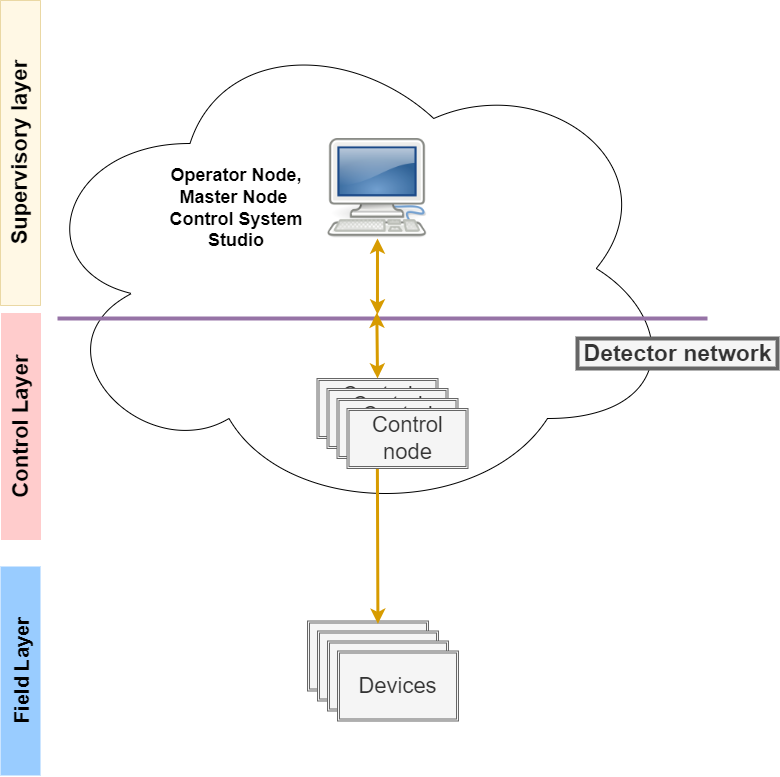
\includegraphics[width=0.5\columnwidth]{Chapter3/Controls/images/example.png}
\caption{General detector control system architecture}
\label{fig_DCS_arch}
\end{figure}

The bottom layer of the Figure \ref{fig_DCS_arch} contains all the process sensors, actuators, and other devices that are connected to the control system via I/O boards and/or field buses. Communication between the field layer and control layer can be of almost any type compatible with the used components, i.e. Ethernet, Modbus TCP, Profibus. The control logic is introduced in \gls{PLC}s and so-called control nodes (single board computers etc.) in the control layer. The supervision layer or supervisory level provides the operators with means of controlling and monitoring the subsystem, for example via command line or a Graphical User Interface (\gls{GUI}) or Operator Interface (\gls{OPI}) \cite{layers}. The three control layers provide an overview of the connections and hardware but don't describe the software part in detail. The \gls{DCS} must provide not only means of communicating between the mentioned layers but also visualization, logging, archiving, and controlling (either in an automated way by a Finite State Machine (\gls{FSM}) or manually). 
\subsection{System requirements}
 The \gls{DCS} for the Silicon Tracking System (\gls{STS}) is being designed taking into consideration the following aspects:
 \begin{itemize}
     \item applications should be easy to run on different operating systems and processor architectures,
     \item horizontal and vertical scalability, when it comes to adding additional computing nodes or applications/Input Output Controllers (\glspl{IOC})/containers,
     \item it should be possible to integrate a sub-system oriented \gls{EPICS}-based \gls{DCS} with higher-level control structures,
     \item the system should be highly available, minimizing the downtimes,
     \item it should be running in a dedicated network (divided into several service-oriented subnets) to have a good overview of the processes and communication between the nodes,
     \item all parameters/process variables should be available in a user-friendly Graphical User Interface (\gls{GUI}). In case of error or malfunction it should be stated clearly by the software where the error happened, what could be the potential risk and what actions need to be taken,
     \item the experiment is supposed to run for about 10 years, excluding the building and commissioning time. The control system should be sustainable and long-term support provided,
     \item there should be reliable means of supervision of processes, containers, and \glspl{IOC}.
 \end{itemize}

The \gls{EPICS} was chosen, as a system that answers most of the needs for the future Detector Control System(s) of the \gls{CBM} experiment. More detailed explanations of how \gls{EPICS} works are described in the next sections. According to \cite{EPICS_DOCS}, the basis attributes of \gls{EPICS} are:
\begin{itemize}
    \item tool based - minimized need for custom coding,
    \item distributed - an arbitrary number of \glspl{IOC} and \glspl{OPI}, as long as the network doesn't the saturation,
    \item event driven - it's designed to be event-driven to the maximum extent possible,
    \item high performance, robust,
    \item scalable,
    \item under constant development (see latest updates related to the Control System Studio and PVA)
\end{itemize}

